\chapter{SU(5), Multiplets, and Proton Decay}

These notes follow Leonard Susskind's lecture on grand unification, with curation by LazyingArt LLC, and they preserve the lecture's order of construction. The subject is not grand unified theories in general, but one concrete example, \(SU(5)\), taken apart slowly enough that we can see both its beauty and its danger. The lecture begins with group theory because the particle story cannot be stated cleanly before the representation theory is in place. Only after that warmup do we fit one Standard Model family into \(SU(5)\), discover the new gauge bosons, and confront the consequence that makes every grand-unified theory live dangerously: proton decay. Supersymmetry enters only at the end, not as a premise, but as a numerical improvement in the running of couplings.

\section{SU(5) as a Concrete Grand-Unification Example}

The lecture opens by narrowing the ambition. We are not going to survey all grand unified theories. We are going to take one theory, \(SU(5)\), and see what makes it tick, what it predicts, and what can go wrong.

The structural claim is that the Standard Model gauge group fits naturally inside a larger simple group:
\begin{equation}
SU(3)\times SU(2)\times U(1)\subset SU(5).
\end{equation}
So the subject is, from the start, an exercise in group theory. We are looking for a single symmetry that contains the separate color and electroweak symmetries as substructures.

The lecture is equally careful about supersymmetry. There is no deep logical statement here that supersymmetry implies grand unification, or conversely that grand unification implies supersymmetry. The point is more modest and more empirical: if one puts the two ideas together, some numerical fits get better.

That is why the lecture pauses before talking about particles and says, in effect: before we do that, we need a little group theory. Particle multiplets are group representations. If we want to classify the multiplets, we must first classify the representations.

\section{Representations of \(SU(N)\): \(N\), \(\bar N\), and Tensor Products}

For \(SU(N)\), the defining representation is simply the space of \(N\)-component complex columns,
\begin{equation}
\psi=
\begin{pmatrix}
\psi_1\\
\psi_2\\
\vdots\\
\psi_N
\end{pmatrix},
\end{equation}
acted on by \(N\times N\) special unitary matrices. In components,
\begin{equation}
\psi'_i=U_{ij}\psi_j.
\end{equation}
This is the \(N\)-dimensional representation usually denoted just by \(N\).

The first new representation we can make is the complex conjugate one. If we take \(\psi_i^*\), then the transformation law is
\begin{equation}
\psi_i^{*\prime}=U_{ij}^*\psi_j^*.
\end{equation}
This is the conjugate representation \(\bar N\). The lecture stresses that \(N\) and \(\bar N\) are both \(N\)-dimensional, and that there is an element of convention in deciding which one we call the particle representation and which one the antiparticle representation. Once we make that choice, however, the bookkeeping must remain fixed.

The next move is the one the lecture announces with the question, ``What else can you do?'' Put down two objects that each transform as \(N\). If one is described by \(\psi_i\) and the other by \(\phi_j\), then the combined state is described by a two-index object
\begin{equation}
\psi_{ij}=\psi_i\phi_j,
\end{equation}
with \(N^2\) components. The group acts on each index separately:
\begin{equation}
\psi'_{ij}=U_{ik}U_{j\ell}\psi_{k\ell}.
\end{equation}
This is the tensor product \(N\otimes N\).

At this point the lecture introduces the key new word: irreducible. The full \(N^2\)-dimensional space is usually reducible. What that means is that there are linear combinations of the \(\psi_{ij}\) that transform among themselves and do not get mixed with the rest. Those smaller closed sectors are themselves representations.

The warmup example is ordinary spin. For \(SU(2)\), the defining doublet may be thought of as the two spin states \(u\) and \(d\). Two such doublets give four raw states, but those four states reorganize into irreducible pieces. That is the bridge from abstract tensor products to familiar physics.

\section{Symmetric and Antisymmetric Two-Index States}

The first clean split of \(N\otimes N\) is into symmetric and antisymmetric tensors. The board at this stage is worth keeping, because it shows the moment when the abstract two-index object is turned into a precise condition.

\begin{figure}
\centering

\includegraphics[width=0.72\textwidth]{lecture_10_figure_02.png}
\caption{The symmetric two-index condition as it appears on the board.}
\end{figure}

The symmetric sector is defined by
\begin{equation}
\psi_{ij}=\psi_{ji},
\end{equation}
while the antisymmetric sector satisfies
\begin{equation}
\psi_{ij}=-\psi_{ji}.
\end{equation}
What matters is that these two sectors do not mix under the group action. Indeed, if \(\psi_{ij}=\pm\psi_{ji}\), then
\begin{align}
\psi'_{ji}
&=U_{jk}U_{i\ell}\psi_{k\ell} \\
&=U_{ik}U_{j\ell}\psi_{\ell k} \\
&=\pm U_{ik}U_{j\ell}\psi_{k\ell} \\
&=\pm \psi'_{ij}.
\end{align}
So the symmetric and antisymmetric subspaces are each preserved by the group. That is precisely the sense in which they are separate representations.

Now we specialize to \(SU(2)\), where the doublet is the spin-\(\tfrac12\) representation. Then
\begin{equation}
2\otimes 2 = 3\oplus 1.
\end{equation}
The four raw states are
\[
|uu\rangle,\qquad |ud\rangle,\qquad |du\rangle,\qquad |dd\rangle.
\]
The symmetric combinations are
\begin{align}
|1,1\rangle &= |uu\rangle,\\
|1,0\rangle &= \frac{1}{\sqrt2}\bigl(|ud\rangle+|du\rangle\bigr),\\
|1,-1\rangle &= |dd\rangle,
\end{align}
and they form a triplet: the spin-one multiplet. The antisymmetric combination is
\begin{equation}
|0,0\rangle = \frac{1}{\sqrt2}\bigl(|ud\rangle-|du\rangle\bigr),
\end{equation}
and it is a singlet: the spin-zero state.

This is the lecture's first major payoff. Two spin-\(\tfrac12\) particles do indeed give four raw states, but those four states do not remain a single lump. The group itself sorts them into one triplet and one singlet. That is the pattern we will carry over to larger groups.

\subsection{Question \& Answer}

Why do two \(N\)-plets give \(N^2\) states without violating the exclusion principle?

Because the lecture is not putting two identical fermions into the same complete quantum state. It is explicitly imagining two distinguishable slots: one particle is here, the other is there. Their internal \(SU(N)\) labels are being discussed while position, momentum, and the rest of the quantum numbers are being held in the background. The Pauli principle constrains the full state. Once the two particles are in different places, there is no contradiction in allowing the same internal label on both sides. So the raw counting really is \(N^2\), and only after that counting do we ask how the group reorganizes those states into irreducible pieces.

\section{From \(N\otimes\bar N\) to the Adjoint, and Then to the Five-Plet}

The next tensor product is conceptually different. Instead of particle with particle, we take particle with antiparticle. The board now isolates the point that this mixed product should be regarded as a matrix.

\begin{figure}
\centering

\includegraphics[width=0.62\textwidth]{lecture_10_figure_04.png}
\caption{The mixed product \(N\times \bar N\) re-expressed on the board as a matrix object.}
\end{figure}

The exact board symbol below \(N\times\bar N\) is not perfectly legible, so we use a cautious clean notation:
\begin{equation}
M_{ij}\in N\otimes \bar N.
\end{equation}
The essential point is that the \(N^2\) components can be organized as an \(N\times N\) matrix. Once we do that, the natural decomposition is into trace and traceless parts:
\begin{equation}
M_{ij}
=
\frac{1}{N}(\operatorname{tr}M)\delta_{ij}
+
\left(
M_{ij}-\frac{1}{N}(\operatorname{tr}M)\delta_{ij}
\right).
\end{equation}
The trace part is a singlet. The traceless part is the adjoint representation, so
\begin{equation}
N\otimes\bar N = 1\oplus \mathrm{Adj},
\qquad
\dim\mathrm{Adj}=N^2-1.
\end{equation}
For \(SU(3)\), this is the familiar statement that quark-antiquark quantum numbers split into a singlet and an octet, with the octet furnishing the gluons.

Only now does the lecture turn to \(SU(5)\) itself. We do not begin by trying to unify all three generations. The lecture makes a point of refusing that larger ambition. We focus on one family. For the first family, the relevant fermions are the up and down quarks in three colors, together with the electron and neutrino.

The first five-component multiplet is then
\begin{equation}
\overline{\mathbf 5}
=
\begin{pmatrix}
\nu_L\\
e^-_L\\
\bar d_{rL}\\
\bar d_{gL}\\
\bar d_{bL}
\end{pmatrix}.
\end{equation}
This looks bizarre at first, and the lecture wants it to look bizarre. One should feel the oddity before one explains it away.

There is also a bookkeeping point here. We list only left-handed particles. The antiparticle of a right-handed electron is a left-handed positron, and similarly for the quarks. So the chiral particle content can be recorded using left-handed particles and left-handed antiparticles only. Mass terms are another story: they connect left- and right-handed fields through Higgs couplings, and the lecture explicitly treats that as a separate issue rather than as part of the grand-unified multiplet structure itself.

\paragraph{A note on convention.}
To keep the notation stable, we adopt the standard convention in which one family sits in \(\overline{\mathbf 5}\oplus \mathbf{10}\). The lecture's spoken and board language can sound like the conjugate convention \(\mathbf 5\oplus \overline{\mathbf{10}}\). We therefore keep the representation labels fixed here and translate the lecture's conjugation language when needed, instead of silently drifting with it.

\subsection{Question \& Answer}

Why does the \(SU(5)\) multiplet contain \(d\)-anti-quarks rather than \(d\)-quarks?

The lecture answers this by returning to the generators of the group. For \(SU(N)\), the generators are Hermitian and traceless. A clean way to see the tracelessness is to look infinitesimally:
\begin{equation}
U(\epsilon)=e^{i\epsilon T}.
\end{equation}
Because \(U(\epsilon)\in SU(N)\), it has determinant one:
\begin{equation}
1=\det U(\epsilon)=\det e^{i\epsilon T}=e^{i\epsilon\,\operatorname{tr}T}.
\end{equation}
For arbitrary \(\epsilon\), this implies
\begin{equation}
T^\dagger=T,\qquad \operatorname{tr}T=0.
\end{equation}

Electric charge must be represented by one of the generators or, more precisely, by a linear combination of them. Therefore the charges within a single multiplet must sum to zero. To display the lecture's point cleanly, we may write the charge operator on the five-component column as
\begin{equation}
Q=\mathrm{diag}\!\left(0,-1,\frac13,\frac13,\frac13\right),
\qquad
\operatorname{tr}Q=0.
\end{equation}
Indeed,
\begin{equation}
0+(-1)+3\left(\frac13\right)=0.
\end{equation}
If we had tried to place \(d\)-quarks rather than \(\bar d\)-quarks in this multiplet, the sum would have been
\[
0+(-1)+3\left(-\frac13\right)=-2,
\]
and electric charge could not be embedded into the traceless generators in the way the lecture requires. That is why the odd assignment is not a decorative flourish. It is forced by the group theory.

\section{The Antisymmetric Matrix and the Remaining Fermions}

The five-plet is clearly not the whole family. Where are the up quarks? Where is the positron? Where do the remaining fields go? The lecture does not answer this by handing us the finished table. Instead it performs, as Susskind says, a bit of gymnastics.

The board next turns to the conjugate five-component column with quantum numbers
\begin{equation}
\chi=
\begin{pmatrix}
\bar\nu\\
e^+\\
d_r\\
d_g\\
d_b
\end{pmatrix}.
\end{equation}
The overbar on the representation label is not the important point here; the important point is the quantum numbers. This column is an auxiliary device for doing the group theory, not a second physical five-plet that we are declaring by fiat. The move is to form the antisymmetric square of this object.

So we introduce a matrix \(\Psi_{ij}\) satisfying
\begin{equation}
\Psi_{ij}=-\Psi_{ji},
\qquad
\Psi_{ii}=0.
\end{equation}
The diagonal entries vanish, the lower triangle is fixed by the upper triangle, and therefore the number of independent entries is
\begin{equation}
\frac{5\cdot 4}{2}=10.
\end{equation}
That is the ten-dimensional multiplet we were looking for.

The board evidence is particularly useful at this stage because it shows the full \(2\oplus 3\) organization.

\begin{figure}
\centering

\includegraphics[width=0.86\textwidth]{lecture_10_figure_05.png}
\caption{The antisymmetric \(5\times 5\) matter matrix on the board, with its visible \(2\oplus 3\) block structure.}
\end{figure}

A clean reconstruction, faithful to the lecture's content while not pretending that every obscured sign is legible on the board, is
\begin{equation}
\Psi \sim
\left(
\begin{array}{cc|ccc}
0 & e^+ & d_r & d_g & d_b\\
-e^+ & 0 & u_r & u_g & u_b\\
\hline
-d_r & -u_r & 0 & \bar u_b & \bar u_g\\
-d_g & -u_g & -\bar u_b & 0 & \bar u_r\\
-d_b & -u_b & -\bar u_g & -\bar u_r & 0
\end{array}
\right),
\qquad
\Psi_{ij}=-\Psi_{ji}.
\end{equation}
The lower \(3\times 3\) block is the least secure part of the board image at the level of signs. The robust content is the antisymmetry, the \(2\oplus 3\) decomposition, and the placement of the \(\bar u\)-type entries in the color-color block.

The lecture then uses the standard color trick. An antisymmetric pair of colors behaves as an anti-color. Thus the antisymmetric color pairs carry the quantum numbers of \(\bar u_r\), \(\bar u_g\), and \(\bar u_b\). With that understood, the remaining fermions fall into place. One family now fits neatly into
\begin{equation}
\overline{\mathbf 5}\oplus \mathbf{10}.
\end{equation}

It is also worth keeping the block structure in a cleaned schematic form, because this is exactly the layout on which the gauge-boson action will later be read. The diagram below is not a replacement for the board image. It is a clarification of the same board logic.

\begin{figure}
\centering
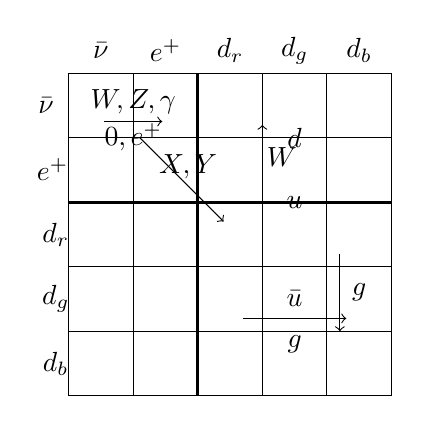
\begin{tikzpicture}[scale=0.82]
\draw (0,0) grid (5,5);
\draw[line width=1.1pt] (0,3) -- (5,3);
\draw[line width=1.1pt] (2,0) -- (2,5);

\node at (0.5,5.35) {$\bar\nu$};
\node at (1.5,5.35) {$e^+$};
\node at (2.5,5.35) {$d_r$};
\node at (3.5,5.35) {$d_g$};
\node at (4.5,5.35) {$d_b$};

\node at (-0.35,4.5) {$\bar\nu$};
\node at (-0.25,3.5) {$e^+$};
\node at (-0.2,2.5) {$d_r$};
\node at (-0.2,1.5) {$d_g$};
\node at (-0.2,0.5) {$d_b$};

\node at (1,4) {$0,e^+$};
\node at (3.5,4) {$d$};
\node at (3.5,3) {$u$};
\node at (3.5,1.5) {$\bar u$};

\draw[->] (0.55,4.25) -- (1.45,4.25);
\node at (1.0,4.55) {$W,Z,\gamma$};

\draw[->] (2.7,1.2) -- (4.3,1.2);
\node at (3.5,0.8) {$g$};

\draw[->] (1.1,4.0) -- (2.4,2.7);
\node at (1.85,3.55) {$X,Y$};

\draw[->] (3.0,3.2) -- (3.0,4.2);
\node at (3.3,3.7) {$W$};

\draw[->] (4.2,2.2) -- (4.2,1.0);
\node at (4.5,1.6) {$g$};
\end{tikzpicture}
\caption{A schematic of the same \(2\oplus 3\) matrix layout: once the blocks are fixed, the gauge bosons act as horizontal or vertical shifts.}
\end{figure}

One should pause here in the same place the lecture pauses. This fit is mathematically striking. At the same time it is awkward in precisely the way the lecture wants us to feel: left-handed up quarks and left-handed anti-up quarks sit in one grand-unified structure, while the left-handed electron and left-handed positron live in different pieces. The point is not to smooth over the oddity too quickly.

\section{Gauge Bosons, Leptoquark Transitions, and Proton Decay}

After the break, the lecture turns from bookkeeping to dynamics. We now ask what the gauge bosons do. The answer begins from the same group-theoretic fact as before: gauge bosons live in the adjoint representation. For \(SU(5)\), that means
\begin{equation}
\dim \mathrm{Adj}_{SU(5)} = 5^2-1 = 24.
\end{equation}
But the lecture does not present them as a list of twenty-four fields. It presents them as shifts.

In the five-component column, the familiar bosons occupy familiar places. The electroweak bosons act in the upper \(2\times 2\) block. The gluons act in the lower \(3\times 3\) color block. The new ingredients are the gauge bosons that connect the upper two slots with the lower three. Those are the leptoquark bosons traditionally called \(X\) and \(Y\).

The lecture is explicit about their charges but deliberately modest about their names. The boson that connects a \(\bar d\) to an \(e^-\) carries charge \(\pm \tfrac43\), while the one that connects a \(\bar d\) to a neutrino carries charge \(\pm \tfrac13\). Susskind explicitly says he does not remember which label, \(X\) or \(Y\), belongs to which charge assignment. We should preserve that caution. The stable content is the transition pattern together with the charges \(\pm \tfrac43\) and \(\pm \tfrac13\).

There is also an important physical remark in the lecture that should not be dropped: these new bosons carry color. They must, because they connect a color-carrying quark state to a colorless lepton state. In that respect they behave more like quarks than like photons. They can emit and absorb gluons, and one should not think of them as free, isolated particles at accessible scales.

How do these same gauge bosons act on the antisymmetric ten-dimensional multiplet? The lecture's picture is that they act as shifts on one index or the other. If we pretend for a moment that a matrix entry is built from a row label and a column label, then a gauge boson can be emitted from either constituent. Emission from one side gives a horizontal move; emission from the other side gives a vertical move. This is why the block picture in the previous section matters.

The weak bosons therefore do more than take \(\nu\leftrightarrow e^-\) in the five-plet. Acting vertically in the antisymmetric matrix, they also take \(d\to u\), which is of course the standard weak transition responsible for beta decay. Likewise the gluons mix the colors of the \(d\)- and \(u\)-type entries. None of that is new. The new physics comes from the \(X\)- and \(Y\)-type shifts between the upper and lower sectors.

Once those shifts exist, new processes exist. One can turn a quark into a lepton, or a lepton into a quark, inside the same unified gauge structure. That is the physical content of grand unification, and it is also the source of its biggest phenomenological danger.

A standard channel in the lecture is
\begin{equation}
p\to e^+ + \pi^0.
\end{equation}
A secondary possibility, suppressed by an extra electromagnetic factor, is
\begin{equation}
p\to e^+ + \gamma.
\end{equation}
The logic is straightforward. Start with a proton, \(uud\). Use one of the heavy leptoquark bosons to convert a \(d\)-quark into a positron and a \(u\)-quark into an anti-\(u\). The remaining \(u\)-quark is a spectator. The \(u\bar u\) pair can form a neutral pion, or more rarely annihilate to a photon.

This is the lecture's physical climax. The story has turned from ``this is a beautiful fit'' to ``this is dangerous.'' If protons decayed as easily as ordinary unstable particles, nuclei would not survive and neither would we.

\subsection{Question \& Answer}

If the new bosons have ordinary-sized couplings, why does the proton not decay immediately?

The lecture's answer is that the only available lever is the mass of the heavy intermediate boson. The unified theory has one gauge coupling at high energies, and the \(X\)- and \(Y\)-boson couplings are not assumed to be absurdly tiny. So the suppression must come from the propagator.

At the level of a rough Feynman-diagram estimate, the amplitude behaves as
\begin{equation}
\mathcal A(p\to e^+\pi^0)\sim \frac{g^2}{M_X^2},
\end{equation}
where the numerator comes from the two gauge vertices and the denominator from the heavy propagator. Squaring the amplitude gives the rate,
\begin{equation}
\Gamma_p \sim \frac{g^4}{M_X^4},
\end{equation}
up to additional factors involving the proton mass and hadronic matrix elements. The lifetime is the inverse rate,
\begin{equation}
\tau_p\sim \Gamma_p^{-1}.
\end{equation}

The lecture then compares this with the scale of microscopic physics. If everything were of order one in proton units, the natural lifetime would be the light-crossing time of a proton, roughly \(10^{-23}\) seconds. But experimentally one finds only lower bounds, and the lecture quotes the observational scale as roughly
\begin{equation}
\tau_p \gtrsim 10^{33}\ \text{years}.
\end{equation}
So the gap to be explained is enormous. The only way to reconcile the unified interaction with proton stability is to make the exchanged boson extremely heavy:
\begin{equation}
M_X \sim 10^{15}\text{--}10^{16}\,\mathrm{GeV},
\end{equation}
with the lecture settling on the memorable order of magnitude
\begin{equation}
M_X \gtrsim 10^{16}\,\mathrm{GeV}.
\end{equation}

That is why proton decay is not a minor side remark. It is a universal warning sign for grand unification. If one unifies quarks and leptons inside a single simple group, baryon-number-violating processes are very hard to avoid. The theory can survive only if the new bosons sit at a fantastically high scale.

\section{Unification Scale, Running Couplings, and the Supersymmetry Epilogue}

The lecture does not leave the number \(10^{16}\,\mathrm{GeV}\) hanging in isolation. It immediately asks: is that a ridiculous scale? The answer given in the lecture is no. It is still a few orders of magnitude below the Planck scale, and more importantly, there is an independent reason to find it attractive.

First, \(SU(5)\) cannot be an unbroken symmetry of nature. If it were, the \(X\) and \(Y\) bosons would live in the same multiplet as the gluons, the \(W\), the \(Z\), and the photon, and there would be no explanation for the huge mass difference. So the theory requires a separate high-scale Higgs phenomenon that breaks the full symmetry, roughly by splitting the upper \(2\)-block from the lower \(3\)-block. Above that scale, however, the difference between the heavy and light gauge bosons becomes negligible, and the full \(SU(5)\) symmetry should be restored as a good approximation.

That is what the lecture means by the unification scale. At energies far above \(M_X\), even the \(X\)- and \(Y\)-boson masses become negligible, and the world should begin to look \(SU(5)\)-invariant. So we ask where the running couplings seem to converge.

The lecture phrases this graphically. Instead of plotting the couplings themselves, it plots their inverses against \(\log \mu\):
\begin{equation}
\alpha_1^{-1}(\mu),\qquad \alpha_2^{-1}(\mu),\qquad \alpha_3^{-1}(\mu).
\end{equation}
The three lines do not meet perfectly in the minimal nonsupersymmetric picture, but they come tantalizingly close. The near-crossing occurs at
\begin{equation}
\mu \sim 10^{15}\text{--}10^{16}\,\mathrm{GeV},
\end{equation}
the same range that proton stability was already suggesting.

So the lecture closes the circle. Proton decay forces the new leptoquark bosons to be extremely heavy. The running of the Standard Model couplings suggests that the place where the separate gauge couplings begin to look unified is again around \(10^{15}\) to \(10^{16}\,\mathrm{GeV}\). These are not two unrelated numbers.

Supersymmetry then returns as an epilogue, exactly as promised in the opening minute of the lecture. There is no deep theoretical necessity tying it to grand unification. But if one includes the superpartner spectrum in the running, the three coupling lines meet much more cleanly, at roughly the one-percent level. That does not prove either idea. It simply makes the coincidence sharper and therefore harder to ignore.

The lecture also remarks, briefly, that a still larger unifying group can package the matter even more neatly. In the theory commonly written \(SO(10)\), one family together with a right-handed neutrino fits into a single sixteen-dimensional multiplet. But that is only a glimpse of a larger story. The lecture itself remains centered on \(SU(5)\).

\section{Summary}

The lecture unfolds in a deliberate order. First we build just enough representation theory to speak cleanly: the defining representation \(N\), the conjugate representation \(\bar N\), the symmetric and antisymmetric pieces of \(N\otimes N\), and the singlet plus adjoint decomposition of \(N\otimes \bar N\). Without that apparatus, the later particle assignments would look arbitrary.

Then the physical content appears. One Standard Model family fits into the grand-unified pattern
\[
\overline{\mathbf 5}\oplus \mathbf{10},
\]
with the five-component multiplet containing \(\nu\), \(e^-\), and the three \(\bar d\)'s, and the antisymmetric ten-dimensional matrix carrying the remaining fermions. The same group structure also forces new gauge bosons that connect quarks and leptons.

That is the beauty and the danger in one stroke. The new bosons make proton decay possible. Proton stability then drives their masses up to the neighborhood of \(10^{16}\,\mathrm{GeV}\). The running couplings suggest that this same scale is where the broken \(SU(5)\) symmetry begins to re-emerge. Supersymmetry does not create that logic, but it sharpens its numerical form. The lecture leaves us with precisely that tension: a remarkably elegant group-theoretic picture, and a universe that permits it only if the most dangerous new processes are pushed almost unimaginably far away.